\documentclass{article}
\usepackage[utf8]{inputenc}

\title{TT3010 - Audio technology and room acoustics. \newline Exercise 6 - Music scales \newline Solutions}


\author{Jan Arne Bosnes}
\date{\today}

\usepackage{natbib}
\usepackage{graphicx}
\usepackage{multicol}
\usepackage{gensymb}
\usepackage{float}
\usepackage{wasysym}
%\usepackage{amsmath}


\begin{document}

\maketitle

All tasks are based on chapter 9 in Rossings "Science of Sound" \cite{rossing}. 
It is recommended that the student will try to do every task, but tasks marked \textit{Mandatory} are to be handed in for approval (online). Deadline is November 23 at 16:00.

\section{}

The ratio of frequencies for a semitone in the scale of equal temperament is given as follows:

\begin{equation}
    f_2/f_1 = 2^{1/12} = 1.05946
\end{equation}

For a major third, we know that it has a step of four semitones, so the ratio of frequencies can be obtained by multiplying the semitone of equal temperament four times:
\begin{equation}
    f_2/f_1 = \left( 2^{1/12} \right)^4 =2^{(4\cdot \frac{1}{12})}= 1.260
\end{equation}
This number is very close to 5/4 = 1.25, and therefore the fifth harmonic of the lower tone is very close to the fourth harmonic of the higher tone, and gives a perception of {\em consonance}.

A minor third has a step of three semitones. Then the ratio of frequencies, for a minor third in equal temperament, can be obtained by multiplying the ratio of the frequencies for a semitone of equal temperament 3 times:
\begin{equation}
    f_2/f_1 = \left( 2^{1/12} \right)^3 = 2^{(3 \cdot \frac{1}{12})} = 1.189
\end{equation}
%
\section{}

So, the rate will grow by 1.059 which we know is about the same as $2^{\frac{1}{12}}$ = the step for one semi-tone. For twelve years, we will then get a step which is the same as moving twelve sem-tones = one octave. Therefore, the ratio should be 2. Numerically, we can check: $\left( 2^{1/12} \right)^{12} = 2^{\left(\frac{1}{12}\cdot 12\right)} = 2^1=2$.

\section{}

Using table 9.2, you will find the following.

\begin{itemize}
    \item Center frequency 31.5 Hz is closest to the frequency $B_0=30.868$ Hz on the musical scale.
    \item Center frequency 63 Hz is closest to the frequency $B_1=60.735$ Hz on the musical scale.
    \item Center frequency 125 Hz is closest to the frequency $B_2=123.47$ Hz on the musical scale.
    \item Center frequency 250 Hz is closest to the frequency $B_3=246.94$ Hz on the musical scale.
    \item Center frequency 500 Hz is closest to the frequency $B_4=493.88$ Hz on the musical scale.
    \item Center frequency 1000 Hz is closest to the frequency $B_5=987.77$ Hz on the musical scale.
    \item Center frequency 2000 Hz is closest to the frequency $B_6=1975.5$ Hz on the musical scale.
    \item Center frequency 4000 Hz is closest to the frequency $B_7=3951.5$ Hz on the musical scale.
    \item Center frequency 8000 Hz is closest to the frequency $B_8=7902.1$ Hz on the musical scale.
\end{itemize}
%
\section{}

Using table 9.2, you will find the following.

\begin{itemize}
    \item The touch-tone frequency 697 Hz is closest to the frequency $F_5=698.46$ Hz on the musical scale.
    \item The touch-tone frequency 770 Hz is closest to the frequency $G_5=783.99$ Hz on the musical scale.
    \item The touch-tone frequency 850 Hz is closest to the frequency $G_5^\#$ Hz on the musical scale.
    \item The touch-tone frequency 941 Hz is closest to the frequency $A_5^\# = 932.33$ Hz on the musical scale.
    \item The touch-tone frequency 1209 Hz is closest to the frequency $D_6^\# = 1244.5$ Hz on the musical scale.
    \item The touch-tone frequency 1337 Hz is closest to the frequency $ E_6 = 1318.5$ Hz on the musical scale.
    \item The touch-tone frequency 1477 Hz is closest to the frequency $F_6^\# $ Hz on the musical scale.
\end{itemize}
%
\section{}

The fifth has the ratio 3:2 and the fourth has the ratio 4:3. We will then get the following ratio:

\begin{equation}
    \frac{3}{2} \cdot \frac{4}{3} = \frac{4}{2} = \frac{2}{1}
\end{equation}

Which is the corresponding ratio to an interval of one whole octave.

We use the same procedure when considering a major sixth (5:3) and a minor third(6:5).

\begin{equation}
    \frac{5}{3}\cdot \frac{6}{5} = \frac{6}{3} = \frac{2}{1}
\end{equation}

So, a major sixth and a minor third correspond to an octave.


\section{}

The ratio of the interval C : G correspond to a ratio 3:2, which is a perfect fifth.

The ratio of the interval E : B as follows,

\begin{equation}
    \frac{E}{B}=\frac{(\frac{E}{C})}{(\frac{B}{C})} = \frac{3}{2}
\end{equation}

which is a perfect fifth.

The ratio of the interval F : C as follows,

\begin{equation}
    \frac{F}{C}=\frac{(\frac{F}{C})}{(\frac{C}{C})} = \frac{3}{2}
\end{equation}

which is a perfect fifth.

The ratio of the interval G : D as follows,

\begin{equation}
    \frac{G}{D}=\frac{(\frac{G}{C})}{(\frac{D}{C})} = \frac{3}{4}
\end{equation}

which is not a perfect fifth.

The ratio of the interval A : E as follows,

\begin{equation}
    \frac{A}{F}=\frac{(\frac{A}{C})}{(\frac{E}{C})} = \frac{4}{5}
\end{equation}

which is not a perfect fifth.

The ratio of the interval D : A as follows,

\begin{equation}
    \frac{D}{A}=\frac{(\frac{D}{C})}{(\frac{A}{C})} = \frac{40}{27}
\end{equation}

which is not a perfect fifth.

\section{}

The formula for the conversion of cents to a frequency ratio is

\begin{equation}
    R_{cent}=10^{(cent \cdot \log(2))/1200}
\end{equation}

So, for 25 cent, $R_{25}=1.0145$, which is the frequency ratio.

For $A_4$, the corresponding frequency is 440 Hz. The new added frequency with 25 cents are $f_2=R_{25}\cdot f_{A4}=446.38 Hz$. So, adding 25 cent to $A_4$ gives us $A_4+25 = 440 \ Hz \ + \ 446.38 \ Hz = 886.38 \ Hz $ and subtracting 25 cents gives us $A_4 - 25 ? 440 \ Hz \ - 446.38 \ Hz \ = 6.38 \ Hz$

So I (Elise) don't understand totally this answer so this is my way of doing it :

\begin{equation}
    f+25cent=f*2^{\frac{25}{1200}}=446Hz
\end{equation}
\begin{equation}
    f-25cent=f*2^{\frac{-25}{1200}}=433.7Hz
\end{equation}

\section{}

The formula for the conversion of frequency ratio to cents is,

\begin{equation}
    I = \frac{1200}{\log{2}} \log{R}\ {\rm cents}
\end{equation}
where $R$ is the ratio of the frequencies. Now the standard C's  from table 9.2 that are near the frequencies 128 Hz, 256 Hz and 512 Hz and $C_3$ with frequency 130.81 Hz, $C_4$ with frequency 261.63 Hz, and $C_5$ with frequency 535.25 Hz.

The frequency ratio for 128 Hz will then be $R=\frac{130.81 \ Hz}{128 \ Hz}$.

Using the conversion formula, we will get,

\begin{equation}
    I = \frac{1200}{\log{2}} \log{\frac{130.81}{128}} = 37.67 \ {\rm cents} 
\end{equation}

So, the tuning fork of frequency 128 Hz is 37.67 cents flat compared to the standard frequency of 130.81 Hz.

The frequency ratio for 256 Hz will then be $R=\frac{261.63 \ Hz}{256 \ Hz}$.

Using the conversion formula, we will get,

\begin{equation}
    I = \frac{1200}{\log{2}} \log{\frac{261.63}{256}} = 37.67 \ {\rm cents} 
\end{equation}

So, the tuning fork of frequency 256 Hz is 37.67 cents flat compared to the standard frequency of 261.63 Hz.

The frequency ratio for 512 Hz will then be $R=\frac{523.25 \ Hz}{512 \ Hz}$.

Using the conversion formula, we will get,

\begin{equation}
    I(cent) = 
    \frac{1200}{\log{2}} \log{\frac{532.25}{512}} = 37.67 \ {\rm cents} 
\end{equation}

So, the tuning fork of frequency 512 Hz is 37.67 cents flat compared to the standard frequency of 523.25 Hz.

An other way to see this (same equations but for me it's easier to understand) is :
a cent measures the ratio between two frequencies (like an octave, a tone...), so if with have n cent this corresponds to 
\begin{equation}
    \frac{f_1}{f_2} = 2^{n/1200}
\end{equation}
Since we want to find n, the number of cents we can isolate it
\begin{equation}
   log_2( \frac{f_1}{f_2})*1200 = n
\end{equation}
$log_2$ is not very practical for the calculations so I switch to $log_{10}$

\begin{equation}
   log_2( \frac{f_1}{f_2})*1200 = log_{10}( \frac{f_1}{f_2})*1200/log_{10}(2)=n
\end{equation}
\begin{figure}[H]
    \centering
    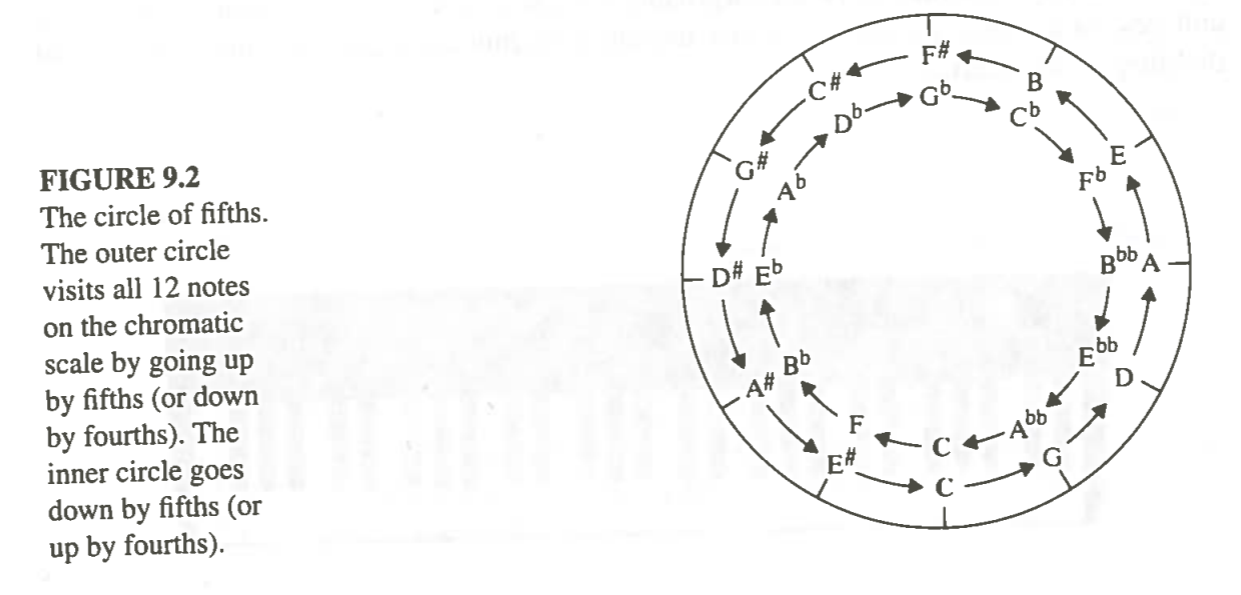
\includegraphics{figures/oving9_1.png}
    \label{fig:1}
\end{figure}

\begin{figure}[H]
    \centering
    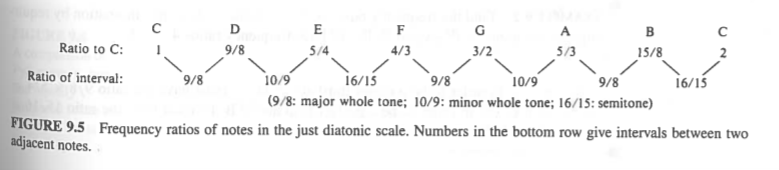
\includegraphics[scale=1.5]{figures/oving9_4.png}
\end{figure}

\begin{figure}[H]
    \centering
    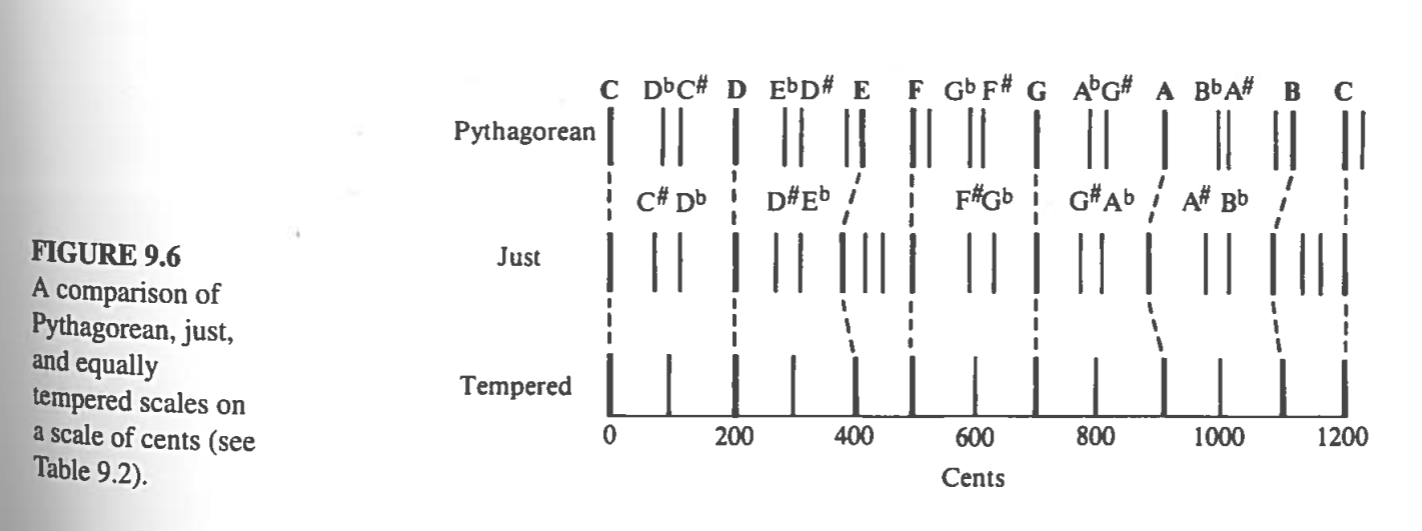
\includegraphics{figures/oving9_2.png}
    \label{fig:2}
\end{figure}

\begin{figure}[H]
    \centering
    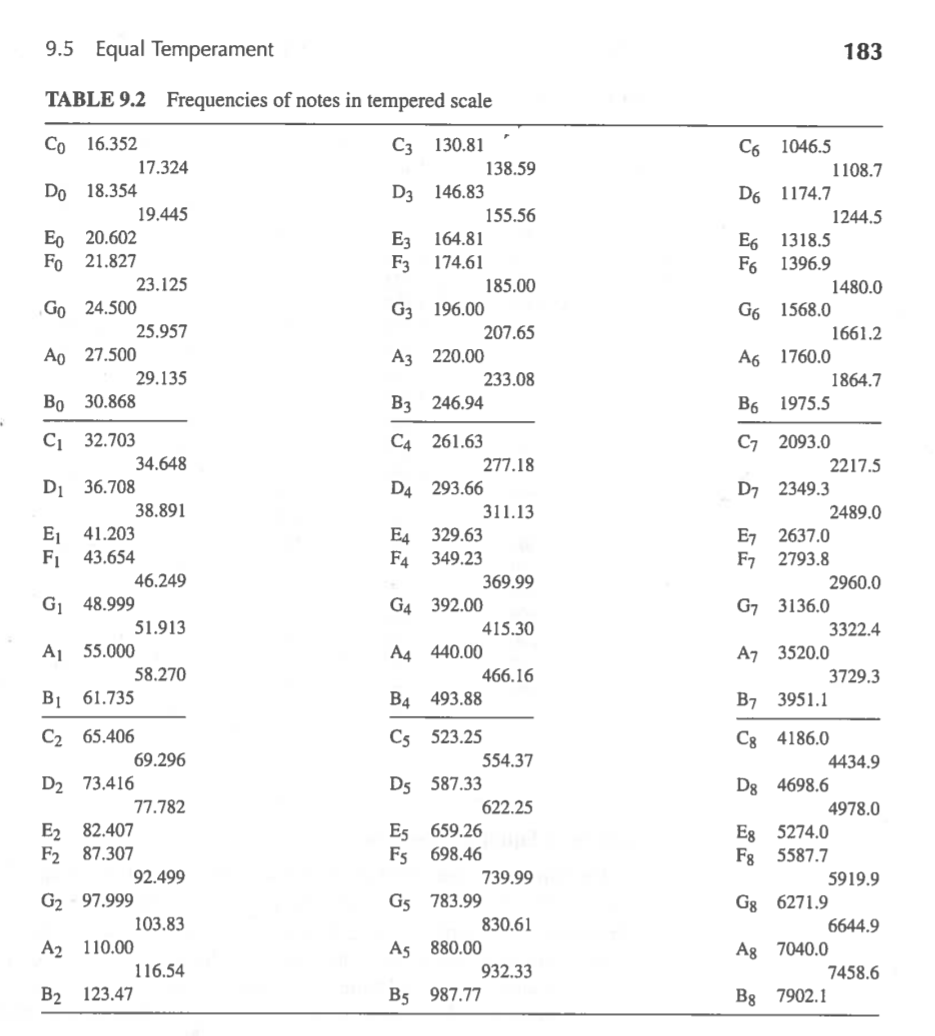
\includegraphics[scale=1.3]{figures/oving9_3.png}
    \label{fig:3}
\end{figure}

\end{document}

